\documentclass[bibliography=totoc,captions=tableheading,titlepage=firstiscover]{scrartcl}

\usepackage{scrhack}

\usepackage[aux]{rerunfilecheck}

\usepackage{polyglossia}
\setmainlanguage{german}

\usepackage[backend=biber,]{biblatex}
\addbibresource{lit.bib}
\usepackage{amsmath}
\usepackage{amssymb}
\usepackage{mathtools}

\usepackage{fontspec}

\usepackage[
  math-style=ISO,
  bold-style=ISO,
  sans-style=italic,
  nabla=upright,
  partial=upright,
]{unicode-math}

\usepackage[
  locale=DE,
  separate-uncertainty=true,
  per-mode=reciprocal,
  output-decimal-marker={,},
]{siunitx}

\usepackage{float}
\floatplacement{figure}{htbp}
\floatplacement{table}{htbp}

\usepackage[
  labelfont=bf,
  font=small,
  width=0.9\textwidth,
]{caption}

\usepackage{graphicx}
\usepackage{grffile}

\usepackage{booktabs}

\usepackage[
  unicode,
]{hyperref}

\usepackage{bookmark}

\begin{document}
  \section{Theorie}
  \section{Durchführung}
  \begin{figure}[H]
    \center
    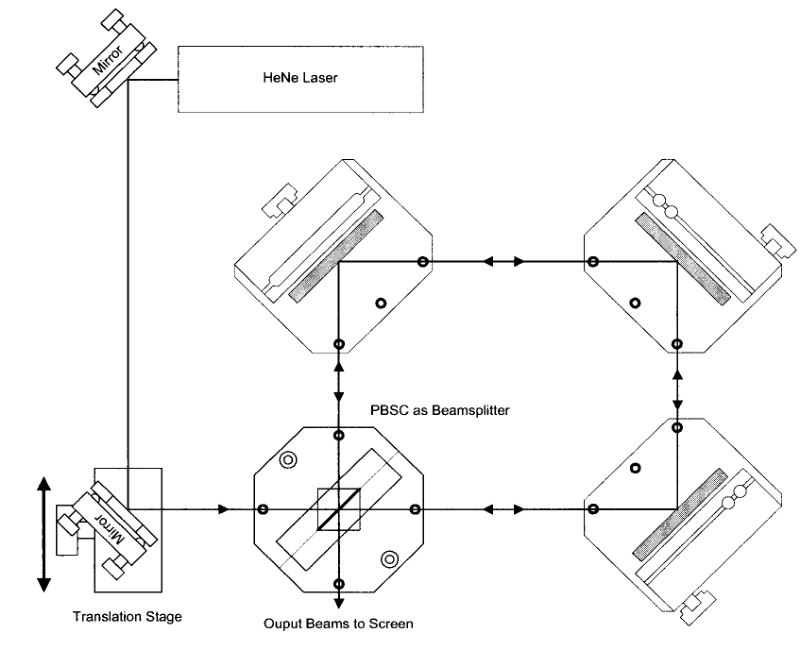
\includegraphics[width=\textwidth]{Versuchsaufbau.JPG}
    \label{fig:aufbau}
    \caption{Aufbau des Sagnac-Interferometers}
  \end{figure}
  \begin{figure}[H]
    \center
    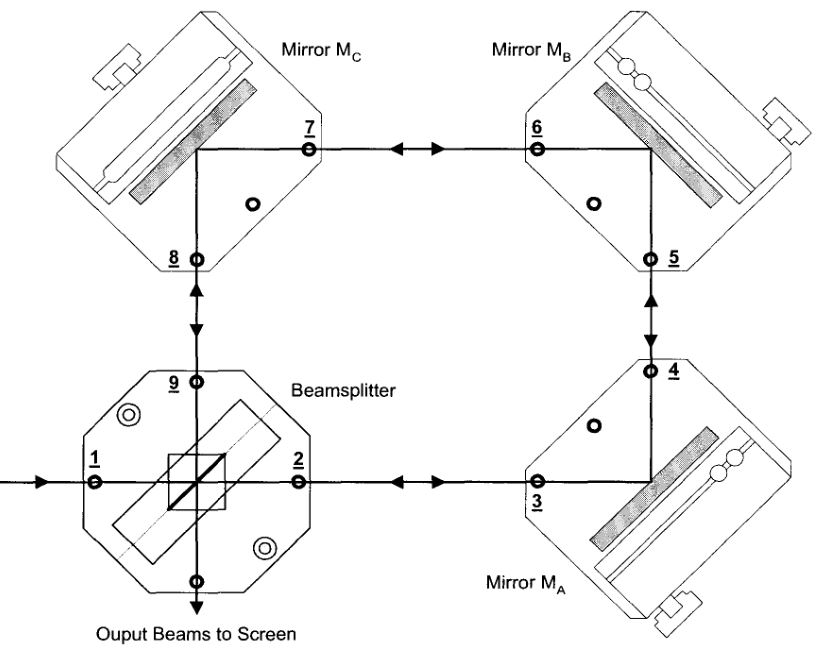
\includegraphics[width=\textwidth]{Strahlengang.JPG}
    \label{fig:bauteilpos}
    \caption{Strahlengang des Sagnac-Interferometers und Montagepunkte der Lochblenden zur Justage}
  \end{figure}
  In den Abbildungen \ref{fig:aufbau} und \ref{fig:bauteilpos} ist der generelle Aufbau des Sagnac Interferometers zu sehen. Hinter dem PBSC aus der Abbildung wird
  zur Messung der Interferenzmuster noch ein weiterer PBSC zur Teilung des Strahls auf 2 Photodioden eingebaut. Die Signale der Dioden werden auf einem Oszilloskop von einander subtrahiert und
  als Differenzsignal visualisiert.
  Zur zusätzlichen Justierung wird der HeNe-Laserstrahl vor dem Auftreffen auf den PBSC noch über 2 Spiegel geleitet. Durch den linken unteren Spiegel kann die Aufteilung des Strahls in hin- und rückläufigen
  Strahl bewirkt werden, was für die späteren Messungen von nöten ist. Zur korrekten Justierung des Strahls auf die Spiegel werden ausserdem Lochblenden verwendet.\\
  Bevor mit der Messung der Intensitätsmaxima und Minima begonnen werden kann, werden nun die die Strahlen im Interferometer korrekt auf die Photodiode
  ausgerichtet.\\
  Anschließend werden die Plättchen in das Interferometer gebracht. Nun wird der Polarisationsfilter, welcher vor Punkt 1 positioniert ist,
  in 10\circ Schritten gedreht. Aus dem auf dem Oszilloskop sichtbaren Referenzsignal lassen sich nun die maximalen und minimalen Intensitäten ablesen, welche entstehen, wenn
  man die Plättchen im Interferometer um einen Winkel im Strahl kippt. Aus den gemessenen Daten wird in der Auswertung der Kontrast errechnet.\\
  \\
  Im zweiten Teil des Versuchs soll der Brechungsindex der zuvor bereits verwendeten Plättchen ermittelt werden. Dazu werden die um 10\circ aus der Ebene senkrecht zum Strahl gekippten Plättchen in Laserstrahl des Interferometers eingeführt.
  Anschließend wird die Anzahl der Interferenzmaxima bei einer Rotation um 10 - 11 Grad senkrecht zur Strahlebene in 1 Grad Schritten gemessen.\\
  \\
  Im letzten Teil des Versuchs wird statt der Plättchen eine Gaszelle in den Laserstrahl geschoben und mithilfe einer angeschlossenen Vakuumpumpe evakuiert.
  Hier werden die Anzahl der Counts bei zurück auf Umgebungsdruck steigendem Druck in der Kammer aufgenommen.
\section{Auswertung}
\subsection{Messung des Kontrasts der Apparatur}
Für die Ermittlung des Kontrasts des Interferometer wird ein Laser mit einer Wellenlänge von $\lambda_{vac}=\SI{623.99}{\nano\meter}$ verwendet.
Aus den gemessenen Intensitäten wird dann mithilfe von Formel \eqref{eq:kontrast} der Kontrast berechnet.
Die Messwerte, sowie der berechnete Kontrast sind in Tabelle \ref{tab:Kontrast} zusammengestellt.
Das Maximum des Kontrasts liegt bei einem Winkel von 60\circ.\\
\begin{figure}[H]
  \center
  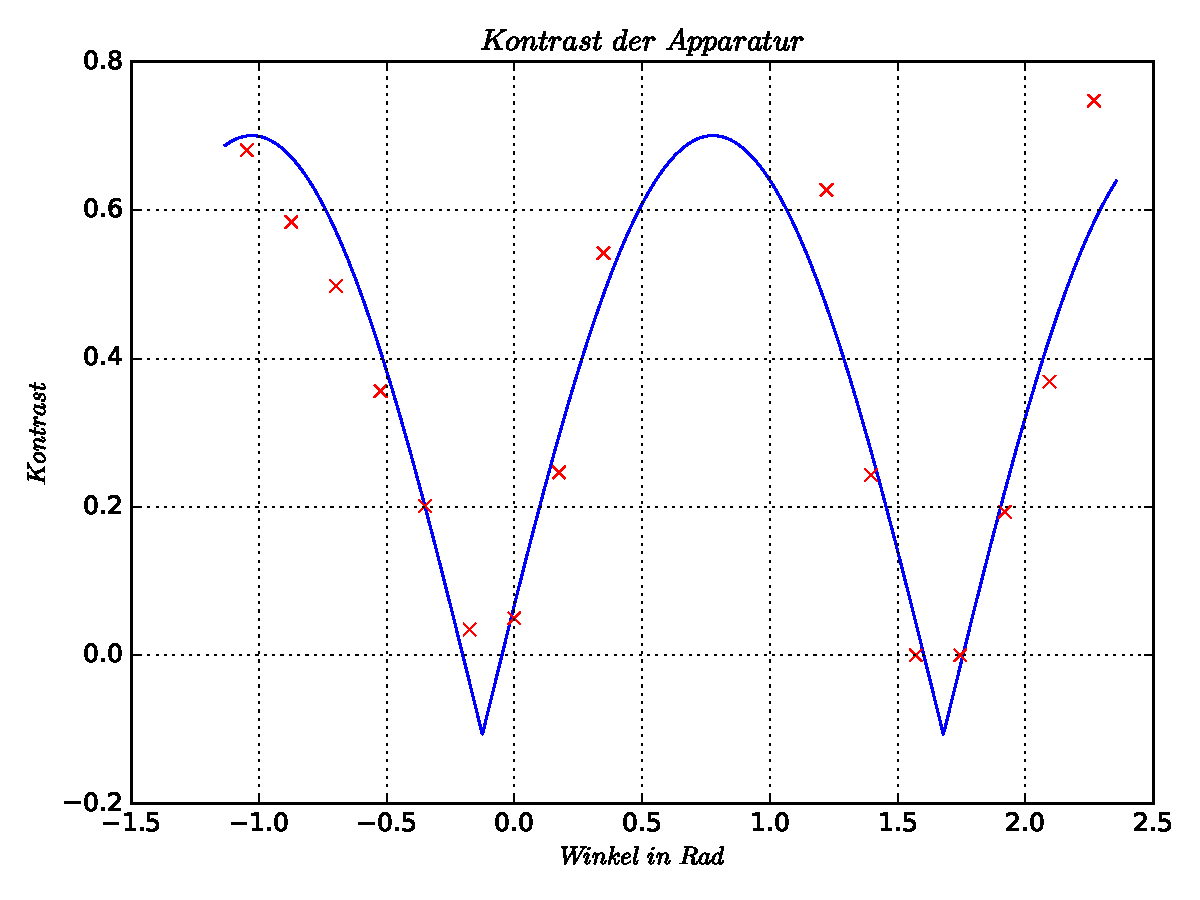
\includegraphics[width=0.65\textwidth]{kontrastplot.pdf}
  \caption{Winkel der Platten und aus den gemessenen Intensitäten errechneter Kontrast.}
  \label{fig:kontrastplot}
\end{figure}
\begin{table}[H]
  \center
  \caption{Zu unterschiedlichen Winkeln gemessene Intensitäten dazu errechneter Kontrast.}
  \label{tab:Kontrast}
\begin{tabular}{c|c|c|c}
  Winkel in Grad& $U_{min}$ in mV& $U_{max}$ in mV& Kontrast\\
  \hline
  -60 &    -1085&       25& 0.6808\\
  -50 &     -975&       25& 0.5841\\
  -40 &  -969.75&   -37.50& 0.4979\\
  -30 &  -969.75&  -281.25& 0.3561\\
  -20 & -1118.75& -1012.50& 0.2013\\
  -10 & -1106.75&  -668.75& 0.0347\\
  0   & -1118.75& -1043.75& 0.0498\\
  10  & -1118.75&  -743.75& 0.2465\\
  20  & -1118.75&  -531.25& 0.5422\\
  30  & -1118.75&  -375.00& 0.9255\\
  40  & -1118.75&  -293.75& 0.95\\
  45  & -1118.75&  -212.50& 0.955\\
  50  & -1118.75&   -87.50& 0.8549\\
  \hline
  60  & -1118.75&   -18.75& 0.9670\\
  \hline
  70  & -1118.75&  -256.25& 0.6273\\
  80  & -1118.75&  -681.25& 0.2431\\
  90  &        -&        -&      0\\
  100 &        -&        -&      0\\
  110 & -1118.75&  -756.25& 0.1933\\
  120 &  -1125.0&  -518.75& 0.3688\\
  130 &  -1125.0&  -162.50& 0.7476\\
\end{tabular}
\end{table}
In \ref{fig:kontrastplot} ist der Kontrast in Abhängigkeit des Drehwinkels der Platten aufgetragen und mithilfe von $curve-fit$ gefitted worden.
Um die Messwerte optimal durch einen Fit zu approximieren wurden die Messwerte zwischen $30^\circ$ und $60^\circ$ aus dem Diagramm entfernt. Bei $90^\circ$ und $100^\circ$ sind beide Intensitäten im Hintergrundrauschen untergegangen, woraus sich der Kontrast von 0 ergibt.\\
\subsection{Berechnung des Brechungsindex der Platten}
  In der Anleitung \cite{Anleitung} finden sich zur Berechnung des Brechungsindex der Platten folgende Herstellerangaben:\\
\begin{center}
  $T = \SI{1}{\milli\meter}$, $n_{\symup{Lit}}=1.35$, $\delta =10$\circ
\end{center}
Anhand dieser Angaben, sowie den gemessenen Werten, wird mithilfe von Formel (???) aus der Theorie der Brechungsindex der Platten errechnet.
Die berechneten Werte sind in Tabelle \ref{tab:plattenindex} einzusehen.\\
\begin{table}[H]
  \center
  \caption{Gemessene Counts bei einer Drehung der Platten um ca. $\theta=10^\circ$ und Mittelwert des berechneten Brechungsindex.}
  \label{tab:plattenindex}
  \begin{tabular}{c|c|c|c}
    Messung& Counts M& Brechungsindex n& Fehler\\
    \hline
    1& 55& 1.049& 0.036\\
    2& 40& 1.038& 0.027\\
    3& 55& 0.750& 1.159\\%Bullshit messung! in den messwerten ist auch n fetter sprung.
    4& 51& 1.015& 0.050\\
    5& 55& 1.015& 0.054\\
    6& 43& 1.036& 0.031\\
    7& 37& 1.023& 0.023\\
    8& 34& 1.034& 0.023\\
  \end{tabular}
\end{table}
\subsection{Berechnung des Brechungsindex von Luft}
In den Tabellen \ref{tab:druckdaten1} und \ref{tab:druckdaten2} sind die mithilfe von Formel \eqref{eq:luft} berechneten Werte des Brechungsindex von Luft bei steigendem Druck zu sehen.
Die Wellenlänge des Lasers beträgt nach wie vor $\lambda_{vac}=\SI{632.99}{\nano\meter}$. Die Länge der Gaszelle ist durch $L=\SI{10}{\centi\meter}$ gegeben.
\begin{table}[H]
  \center
  \caption{Brechungsindex von Luft bei steigendem Druck in 100 mbar Schritten.}
  \label{tab:druckdaten1}
 \begin{tabular}{c|c|c|c}
   $p_1$ in mbar&$n_1$ &$p_2$ in mbar &$n_2$\\
   \hline
   11  &1.000 070 & 12  & 1.000 076\\
   100 &1.000 633 & 100 & 1.000 633\\
   200 &1.001 266 & 200 & 1.001 266\\
   300 &1.001 899 & 300 & 1.001 899\\
   400 &1.002 532 & 400 & 1.002 532\\
   500 &1.003 165 & 500 & 1.003 165\\
   600 &1.003 798 & 600 & 1.003 798\\
   700 &1.004 431 & 700 & 1.004 431\\
   800 &1.005 064 & 800 & 1.005 064\\
   900 &1.005 697 & 900 & 1.005 697\\
   995 &1.006 298 & 995 & 1.006 298\\
 \end{tabular}
\end{table}
\begin{table}[H]
    \center
    \caption{Brechungsindex von Luft bei steigendem Druck in 50 mbar Schritten.}
    \label{tab:druckdaten2}
    \begin{tabular}{c|c|c|c}
      $p_3$ in mbar&$n_3$ &$p_4$ in mbar &$n_4$\\
      \hline
      8  & 1.000 051& 8  & 1.000 051\\
      50 & 1.000 317& 50 & 1.000 317\\
      100& 1.000 633& 100& 1.000 633\\
      150& 1.000 949& 150& 1.000 949\\
      200& 1.001 266& 200& 1.001 266\\
      250& 1.001 582& 250& 1.001 582\\
      300& 1.001 899& 300& 1.001 899\\
      350& 1.002 215& 350& 1.002 215\\
      400& 1.002 532& 400& 1.002 320\\
      450& 1.002 848& 450& 1.002 848\\
      500& 1.003 165& 500& 1.003 165\\
      550& 1.003 481& 550& 1.003 481\\
      600& 1.003 798& 600& 1.003 798\\
      650& 1.004 114& 650& 1.004 114\\
      700& 1.004 431& 700& 1.004 431\\
      750& 1.004 747& 750& 1.004 747\\
      800& 1.005 064& 800& 1.005 064\\
      850& 1.005 380& 850& 1.005 380\\
      900& 1.005 697& 900& 1.005 697\\
      950& 1.006 013& 950& 1.006 013\\
      995& 1.006 298& 995& 1.006 298\\
    \end{tabular}
\end{table}
\printbibliography
\nocite{*}
\end{document}
